\documentclass{article}

\usepackage{mathtools,amsfonts}
\usepackage{enumerate}
\usepackage{fancyvrb}
\usepackage{graphicx}
% \usepackage{fullpage}
\graphicspath{ {./} }

\begin{document}

\begin{center}
  \textbf{\Large <LEVEL> Test <NUMBER> Solutions}
  % LEVEL is Advanced, Intermediate or Beginner
  % NUMBER is the test number: 1, 2, etc.
  \\ \vspace{1em}
  \textbf{\large Stellenbosch Camp 2019}
\end{center}


\begin{enumerate}[1.]

\item %Source of problem
\textit
{
    Tile an $8 \times 8$ chessboard with T-shaped tetrominoes.
}

\textit{Solution}: 
\begin{center}
    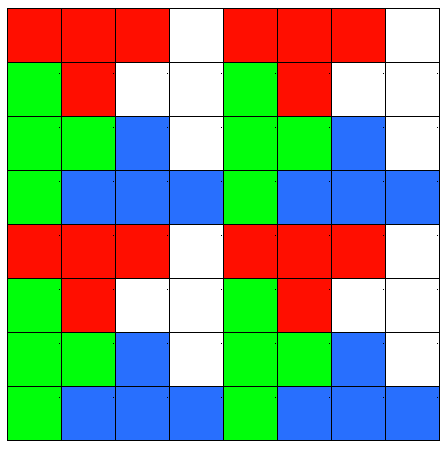
\includegraphics[scale=0.5]{tiling.png}
\end{center}

\item %Source
\textit{}

\textit{Solution}:


\end{enumerate}

\end{document}
